\documentclass{BeamerTemplate}

\title{Module 5 - Statistiques descriptives}

\date{\today}

\begin{document}
\begin{frame}[t]
  \titlepage
\end{frame}

%-------------------------------------------------------------------------------------------------------------------------------------





%%%%%%%%%%%%%%%%%%%%%%%%%%%%%%%%%%%
%%%%%%%%%%%%%%%%%%%%%%%%%%%%%%%%%%%
%%%%%%%%%%%%%%%%%%%%%%%%%%%%%%%%%%%


\section{Introduction}

\begin{frame}[t]{Jeu de données statistique}

Un jeu de données est habituellement constitué de \\\alert{plusieurs observations} de \alert{plusieurs variables}. \\

\medskip
{\small
Exemple d'informations recueillies lors d'un processus de production:

{\scriptsize
\begin{center}
\begin{tabular}{ccccc}\hline
Lot & Luminosité ($lux$) & Catalyseur & Vitesse du mélangeur & Température ($^\circ C$) \\ \hline
1 & 12,0 & Oui & Basse & 17 \\
2 & 13,5 & Non & Moyenne & 15 \\
3 & 11,5 & Non & Haute & 14 \\
4 & 13,0 & Oui & Moyenne & 18 \\
5 & 14,0 & Non & Basse & 21 \\
$\vdots$&$\vdots$&$\vdots$&$\vdots$&$\vdots$\\\hline
\end{tabular}
\end{center}
}

\begin{itemize}
\item Variables qualitatives ou quantitatives (traitées différemment en statistique).
\item Nous étudierons les variables \alert{quantitatives} dans ce cours.
\end{itemize}
}
\end{frame}

\begin{frame}[t]{Décrire avant d'analyser}

Une bonne analyse est précédée d'un \alert{résumé} des
%Avant de commencer à déduire le comportement aléatoire de ces variables à partir des observations, il est bon de \alert{résumer} les
principales caractéristiques de la distribution des observations.

\uncover<2->{
\begin{enumerate}[$\bullet$]
\item mesures de \alert{position}
    {\small\begin{enumerate}[$\circ$]
    \item {\color{gray}{moyenne}}
    \item {\color{gray}{médiane}}
    \item {\color{gray}{autres quantiles}}
    \end{enumerate}}
\item mesures de \alert{dispersion}
    {\small\begin{enumerate}[$\circ$]
    \item {\color{gray}{variance et écart-type}}
    \item {\color{gray}{écart interquartile}}
    \item {\color{gray}{étendue}}
    \end{enumerate}}
\item représentations \alert{graphiques}
    {\small\begin{enumerate}[$\circ$]
    \item {\color{gray}{histogramme}}
    \item {\color{gray}{diagramme en boîte}}
    \item {\color{gray}{diagramme quantile-quantile}}
    \end{enumerate}}
\end{enumerate}
}
\end{frame}

\begin{comment}

\begin{frame}[t]{Types de variables}

{\small
Les variables observées sont généralement de l'un de trois types:
\begin{itemize}
\item<1-> {\bf Variable quantitative:} variable dont la valeur est
un nombre entier ou un nombre réel (p.ex., masse, température, nombre
de craques)
\item<2-> {\bf Variable qualitative:}
 \begin{itemize}
  \item<2-> {\bf Variable qualitative ordinale:} Variable dont la valeur n'est \alert{pas
  une mesure continue ou un dénombrement}, mais pour laquelle les modalités
  peuvent \^etre \alert{ordonnées} (p.ex. une variable ``revenu'' avec modalités
  ``faible'', ``moyen'', ``élevé'')
  \item<3-> {\bf Variable qualitative catégorielle:} Variable dont la valeur n'est \alert{pas
  une mesure continue ou un dénombrement} et pour laquelle les modalités
  \alert{ne peuvent pas \^etre ordonnées} (p.ex. une variable ``Couleur'' avec
  valeurs ``Bleu'', ``Rouge'', ``Noir'', ou une variable ``Région
  administrative'' qui prend les valeurs 1, 2, 3, 4 ou 5)
 \end{itemize}
\end{itemize}
}

\begin{itemize}
\item ``Luminosité'' et ``Température'' sont des variables quantitatives
\item ``Lot'' et ``Catalyseur'' sont des variables qualitatives catégorielles
\item ``Vitesse du mélangeur'' est une variable qualitative ordinale
\end{itemize}

\end{frame}
\end{comment}



\section{Description numérique}

\subsection{Mesures de position}

\begin{frame}[t]{Tendance centrale: moyenne et médiane}

%La caractéristique d'une distribution qui nous intéresse en premier lieu est une mesure de sa \alert{localisation}, plus précisément de sa \alert{\em tendance centrale}.
%Dans la majorité des cas, une telle mesure nous donne une idée d'o\`u se situe le centre, le coeur d'une distribution.

Mesure de position la plus commune: \alert{moyenne échantillonnale} \\
{\small (version empirique de la moyenne théorique d'une population, $\mu$).}

\begin{Boite}{Moyenne échantillonnale}
Soit un échantillon observé $x_1,\ldots,x_n$. \\
Sa moyenne échantillonnale est donnée par
$$\alert{\overline{x}}=\frac{x_1+x_2+...+x_n}{n}=\frac{1}{n}\sum_{i=1}^nx_i.$$
\end{Boite}

\end{frame}
\begin{frame}[t]{Caractéristiques de la moyenne échantillonnale}

\begin{itemize}\itemsep0.1cm
\item Point d'équilibre du diagramme de points
\item Fait intervenir toutes les données dans le calcul
\item Sensible aux valeurs extrêmes
\item Si la somme était répartie également, chaque observation vaudrait $\overline x$
%, tout le monde aurait la valeur moyenne
\item Peut être représentative du groupe... ou non %: ($\overline x = 4 et 46.25$)
\end{itemize}
\vspace{5mm}
\begin{center}
  \begin{tabular}{cc}
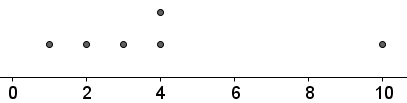
\includegraphics[width=5.1cm]{Images/Module 5/moy.PNG}\hspace{5 mm}& 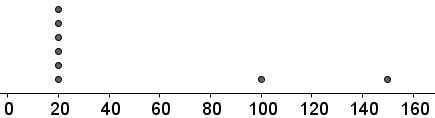
\includegraphics[width=5.1cm]{Images/Module 5/moy2.PNG}\\ &\\
\alert{$\overline x=4$} &\alert{ $\overline x=46,25$}
\end{tabular}  
\end{center}


\end{frame}


\begin{frame}[t]{ }

\centerline{\LARGE\bf \alert{QUIZ !}}
\bigskip

La moyenne d'un échantillon de taille $n=30$ vaut $\overline x =112$. \\
On retire la plus grande et la plus petite observations.
\bigskip

{\bf Vrai ou Faux?}
\bigskip

La moyenne échantillonnale vaut toujours 112.
\vspace{2cm}


\end{frame}
\begin{frame}[t]{Médianes {\it théorique} et {\it échantillonnale}}

Autre mesure de tendance centrale : la médiane.

\medskip
\begin{itemize}


\item \alert{Médiane théorique}: associée à la distribution de $X$, au modèle probabiliste de la population.
\item \alert{Médiane échantillonnale}: calculée à partir d'une série d'observations $x_1,..., x_n$.

\end{itemize}
\vspace{3mm}

\uncover<2->{
\begin{Boite}{Médiane théorique $\widetilde{\mu}$ }

La médiane de la distribution d'une variable aléatoire $X$ est la valeur
$\widetilde{\mu}$ telle que
$$P(X\le \alert{\widetilde{\mu}})=P(X>\alert{\widetilde{\mu}})=\dfrac12.$$

\end{Boite}
}
\end{frame}

\begin{comment}
local({
  .x <- seq(-0.021, 0.83, length.out=10000)
  plotDistr(.x, dbeta(.x, shape1=2, shape2=6), cdf=FALSE, xlab="x",
  ylab="Density", main=paste("Beta Distribution:  Shape 1=3, Shape 2=6"),
  lwd=3,yaxs="i",ylim=c(0,3),las=1)
})

local({
  .x <- seq(9.0005, 12.9995, length.out=10000)
  plotDistr(.x, dunif(.x, min=10, max=12), cdf=FALSE, xlab="x", ylab="Density",
  main=paste("Uniform Distribution:  Minimum=10, Maximum=20"),
lwd=3,yaxs="i",ylim=c(0,0.6),las=1)
})
\end{comment}
\begin{frame}[t]{ }

\centerline{\LARGE\bf \alert{QUIZ !}}
\bigskip

Comment se comparent $\mu$ et $\widetilde\mu$ dans chacune des deux distributions suivantes?
\medskip


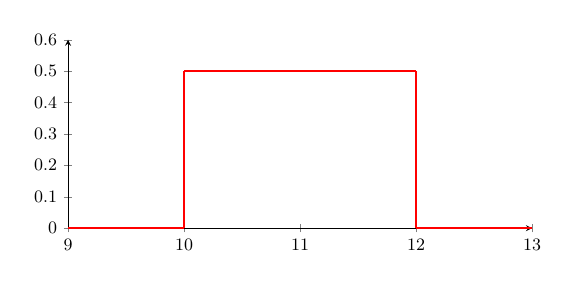
\begin{tikzpicture}[scale = 0.7]
\begin{axis}[
    ymin=0, ymax=0.6,
    xmin=9, xmax=13,
    xtick={9,10,11,12,13},
    ytick={0,0.1,...,0.6},
    axis lines=left,
    width=10cm,
    height=5cm,
    enlargelimits=0,
    tick label style={font=\small}
]
% Courbe rouge (densité stylisée)

\draw[red, thick] (9,0) -- (10,0);  % Avant densité
\draw[red, thick] (10,0) -- (10,0.5);  % Avant densité
\draw[red, thick] (10,0.5) -- (12,0.5);  % Avant densité
\draw[red, thick] (12,0.5) -- (12,0);  % Avant densité
\draw[red, thick] (12,0) -- (13,0);  % Avant densité


\end{axis}
\end{tikzpicture}

\medskip


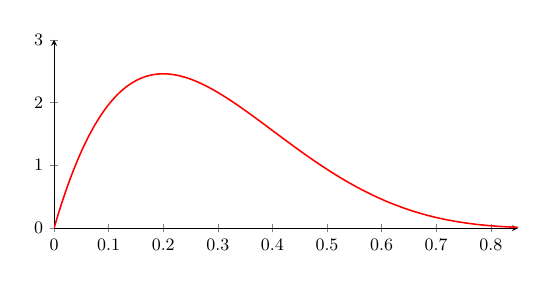
\begin{tikzpicture}[scale = 0.7]
\begin{axis}[
    ymin=0, ymax=3,
    xmin=0, xmax=0.85,
    axis lines=left,
    width=10cm,
    height=5cm,
    enlargelimits=0.,
    tick label style={font=\small}
]
\addplot[domain=0:0.85, red, thick, samples=200] {30 * x * (1 - x)^4};
\end{axis}
\end{tikzpicture}


\end{frame}
\begin{frame}[t]{Notation pour l'échantillon ordonné}

Pour définir les quantiles échantillonnaux (mesures de position dont la médiane fait partie), on doit introduire les \textit{statistiques d'ordre}.

\medskip
\uncover<2->{
%Soit l'échantillon $x_1,\ldots,x_n$ (présenté dans l'ordre de collecte des données).
\begin{Boite}{Statistiques d'ordre}
La $i$-ème statistique d'ordre, notée \alert{$x_{(i)}$}, est la $i$-ème
observation de l'échantillon {\it ordonné} (en ordre croissant).
\end{Boite}

\medskip Exemple 1: \hspace{1cm}
\begin{tabular}{cccc|cccc}
\multicolumn{4}{c|}{Échantillon dans} & \multicolumn{4}{c}{Échantillon}\\
\multicolumn{4}{c|}{l'ordre de collecte} & \multicolumn{4}{c}{ordonné}\\\hline
 $x_1$&$ x_2$&$ x_3$&$ x_4$ & $x_{(1)}$&$ x_{(2)}$&$ x_{(3)}$&$ x_{(4)}$\\[2mm]
 8& 17& 2& 11&     & & &
\end{tabular}
}
\end{frame}
\begin{frame}[t]{Médiane {\it échantillonnale}}

{\small
\begin{Boite}{Médiane échantillonnale}
Valeur centrale de l'échantillon {\it ordonné}, ou la moyenne des deux valeurs centrales dans le cas d'un nombre pair d'observations.

\vspace{-3mm}

\begin{center}\alert{$\widetilde x = x_{(\frac{n+1}{2})}=x_{(0,5n+0,5)}$}\end{center}
\end{Boite}
\begin{itemize}\itemsep-1mm
%\item Point milieu de l'échantillon ordonné
\item Fait intervenir 1 ou 2 données dans le calcul
\item Peu (pas) sensible aux valeurs extrêmes
\item Peut être représentative du groupe... ou non %: ($\widetilde x = 3.5 et 40$)
\end{itemize}
}
\medskip
\begin{center}
    \begin{tabular}{cc}
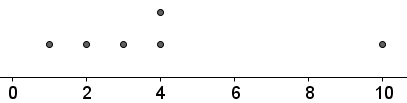
\includegraphics[width=5.1cm]{Images/Module 5/moy.PNG}\hspace{5 mm}& 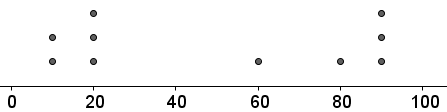
\includegraphics[width=5.1cm]{Images/Module 5/moy3.PNG}\\ &\\
\alert{$\widetilde x=3,5$} &\alert{ $\widetilde x=40$}
\end{tabular}
\end{center}


\end{frame}


\begin{frame}[t]{ }

\centerline{\LARGE\bf \alert{QUIZ !}}
\bigskip

La médiane d'un échantillon de taille $n=30$ vaut $\widetilde x =114$. \\
On retire la plus grande et la plus petite observations.
\bigskip

{\bf Vrai ou Faux?}
\bigskip

La médiane échantillonnale vaut toujours 114.
\vspace{2cm}

\end{frame}
\begin{frame}[t]{Quantiles}
\vspace{-0.6cm}
\begin{Boite}{Quantiles théoriques}
Le quantile théorique d'ordre $a$ ($0\leq a\leq 1$) d'une distribution est la valeur $c_a$ telle que
$$\alert{P(X\le c_a)=a}$$
\end{Boite}

\begin{Boite}{Quantiles échantillonnaux}
Il existe plusieurs définitions des quantiles échantillonnaux. Voici celle que nous utiliserons pour le  quantile échantillonnal d'ordre $a$:
$$\alert{q_a=x_{(an+0,5)}}$$
\end{Boite}

\alert{Si $an+0,5$ n'est pas entier}, on peut faire une interpolation linéaire entre les deux valeurs entières qui l'entourent. On obtient ainsi une moyenne pondérée de $x_{([an+0,5])}$ et $x_{([an+0,5]+1)}$, o\`u $[u]$ est la partie entière de $u$.

\end{frame}
\begin{frame}[t]{Exemple 2}
Considérons un tout petit échantillon:
$$4\quad 3\quad 8\quad 9\quad 6$$

\begin{enumerate}[a)]
\item Quel est le quantile échantillonnal d'ordre $0,3$ de cet échantillon ?
\vspace{1.5cm}


\item  Quel est le quantile échantillonnal d'ordre $0,65$ de cet échantillon?
\end{enumerate}
\vspace{2cm}

\end{frame}

\begin{frame}[t]{Quartiles échantillonnaux}

{\small

\begin{Boite}{Quartiles échantillonnaux}
Les \alert{3 quartiles} séparent l'échantillon en 4 parties de fréquences égales.
\begin{itemize}
\item Le $1^{er}$ quartile est le quantile d'ordre 0,25 ($25^e$ centile): \alert{$Q_1=q_{0,25}$}.
\item Le $2^{e}$ quartile est le quantile d'ordre 0,50 ($50^e$ centile):\\ \alert{$Q_2=\tilde{x}=q_{0,50}$} (la médiane!)
\item Le $3^{e}$ quartile est le quantile d'ordre 0,75 ($75^e$ centile): \\ \alert{$Q_3=q_{0,75}$}.
\end{itemize}
\end{Boite}
}
\end{frame}

\begin{frame}[t]{Exemple 3}
Soit l'échantillon $x_1,\ldots,x_{11}$ suivant:
{\small $5,~ 15,~ 17,~ 15,~  9,~  2,~  2,~ 11,~  4,~  1,~ 4.$}

\vspace{3mm}
Calculez  ses trois quartiles.\\

\end{frame}


\subsection{Mesures de dispersion}

\begin{frame}[t]{Mesures de dispersion}

%Les valeurs observées d'une variable aléatoire ne sont pas toutes égales à sa moyenne.

%\medskip
Deux algorithmes de positionnement par GPS peuvent fournir des localisations moyennes tout aussi précises, mais l’un génère des erreurs beaucoup plus variables d’un point à l’autre. Ainsi, certaines localisations peuvent être très loin de la cible.
Ce manque de constance peut être critique dans des applications comme la navigation de drones ou de véhicules autonomes.

\medskip
En plus des mesures de position, une autre caractéristique importante d'une
distribution est  \alert{la dispersion des valeurs autour du centre de la distribution}.
\end{frame}


\begin{frame}[t]{Étendue échantillonnale}

La mesure la plus simple de la dispersion des données:

\begin{Boite}{Étendue échantillonnale}
Différence entre les valeurs maximale et minimale d'un échantillon:
$$R=x_{(n)}-x_{(1)}$$
\end{Boite}

\begin{itemize}
\item Ne tient compte que des 2 valeurs les plus extrêmes
\item Pas de lien avec les mesures de tendance centrale
\end{itemize}

\end{frame}

\begin{frame}[t]{Variance échantillonnale}

{\small

Rappel: soit $X$ une variable aléatoire quelconque, sa variance est $V(X)=E[(X-\mu)^2]$.

\begin{Boite}{Variance et écart-type échantillonnaux}
La \alert{variance échantillonnale} d'un échantillon $x_1,\ldots,x_n$ est donnée par
$$\alert{s^2}=\frac{1}{n-1}\sum_{i=1}^n(x_i-\bar{x})^2.$$
L'\alert{écart-type échantillonnal} est $\alert{s}=\sqrt{s^2}$.
\end{Boite}
Un truc pour calculer $s^2$ plus rapidement:
$$s^2=\frac{1}{n-1}\sum_{i=1}^n(x_i-\bar{x})^2=\frac{1}{n-1}\left[\sum_{i=1}^nx_i^2-n(\bar{x}\,^2)\right].$$
}
\end{frame}

\begin{frame}[t]{Écart interquartile}

Une mesure alternative de dispersion est \alert{l'écart interquartile}.

\begin{Boite}{Écart interquartile}

L'écart interquartile d'un échantillon est la distance entre le $1^{er}$ et le $3^e$ quartiles :

\vspace{-3mm}
\begin{center}\alert{$EIQ=Q_3-Q_1=q_{0,75}-q_{0,25}$}\end{center}
\end{Boite}
\begin{itemize}
\item L'$EIQ$ est l'étendue de la moitié centrale des données.

\item Exemple 3: l'étendue vaut $R=16$, \\l'écart-type échantillonnal est de $s=5,9$, \\l'écart interquartile est $EIQ=14-2,5=11,5$.
\end{itemize}
\end{frame}




\section{Représentation graphique}
\begin{comment}
png("hist1.png",width=6,height=5,units="in",res=90)
x<-rnorm(100, mean=7, sd=3)
hist(x, main="",yaxs="i",las=1, col="gray",xlab="",ylab="Fréquence")
dev.off()

png("hist2.png",width=6,height=5,units="in",res=90)
y<-rexp(100, rate=1/3)
hist(y, main="",yaxs="i",las=1, col="gray",xlab="",ylab="Densité",breaks=c(0,2,4,8,12,20))
dev.off()

png("hist3.png",width=6,height=5,units="in",res=90)
z<-20-rchisq(100, df=3)
hist(z, main="",yaxs="i",las=1, col="gray",xlab="",ylab="Fréquence")
dev.off()
\end{comment}
\subsection{Histogramme}

\begin{frame}[t]{Histogramme}

\begin{center}
    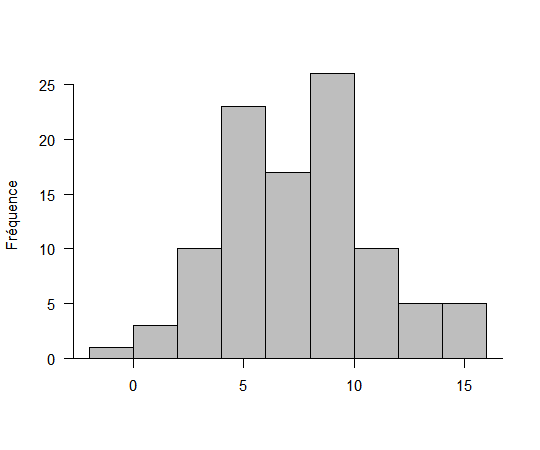
\includegraphics[width=3.5cm]{Images/Module 5/hist1.png}
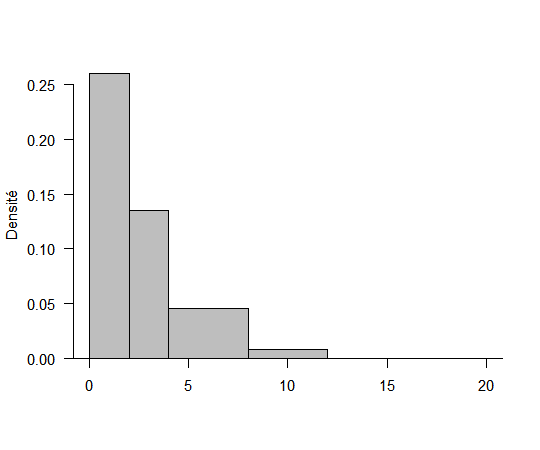
\includegraphics[width=3.5cm]{Images/Module 5/hist2.png}
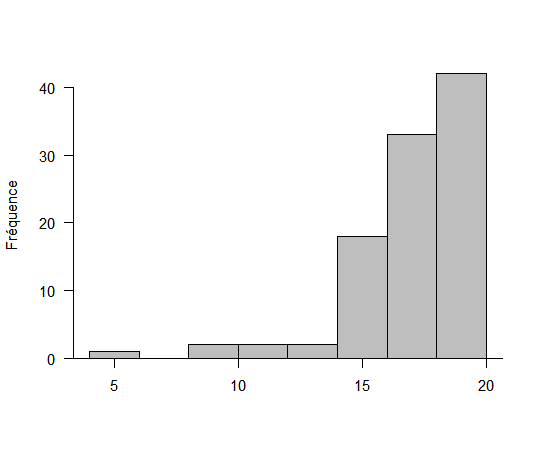
\includegraphics[width=3.5cm]{Images/Module 5/hist3.png}

\end{center}

\begin{itemize}
\item L'histogramme sert à \alert{estimer une fonction de densité à partir d'un échantillon}.
\item Utile pour déterminer si un certain modèle probabiliste est approprié pour la population d'où provient l'échantillon
\item Si l'histogramme est en forme de cloche (\alert{unimodal}  et \alert{symétrique}), nous serons à l'aise avec le postulat de normalité de la population.
    \end{itemize}
\end{frame}

\begin{frame}[t]{Procédure pour tracer un histogramme}

{\small
Soit un échantillon $x_1,\ldots,x_n$.
\begin{itemize}
\item<1-> On divise l'ensemble des valeurs possibles de
$X$ en environ 5 à 10 classes (intervalles de même largeur ou non).% (règle du pouce: prendre un nombre de classes près de $\sqrt{n}$).
\item<2-> Soit $K$, le nombre de classes. On construit le tableau de fréquences contenant: \begin{itemize}
     \item[$n_j$]:  fréquence (absolue), soit le nombre d'observations qui tombent dans la classe $j$, et
     \item[$f_j$] \alert{$=n_j/n$}: fréquence relative de la classe $j$, pour $j=1, ..., K$.
         \end{itemize}
\item<3-> \alert{La surface d'un rectangle doit être proportionnelle à sa fréquence relative. } Soit $\ell_j$, la largeur de la classe $j$, alors $\ell_j\cdot h_j = c\cdot f_j$, avec $c$ constant.

\item<3-> Classes égales:  hauteurs égales aux fréquences absolues ou relatives.

\item<3-> Classes inégales: histogramme de densité ($c=1$), où  $$\alert{h_j=f_j/\ell_j}$$.
\end{itemize}
}
\end{frame}

\begin{frame}[t]{Hauteur des rectangles d'un histogramme}

\begin{center}
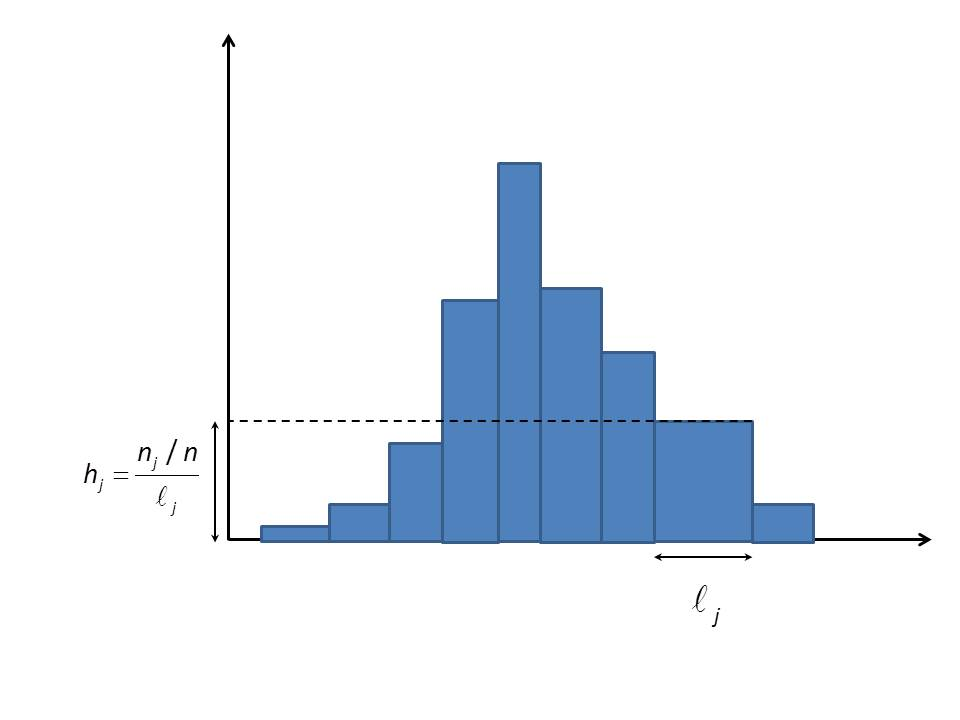
\includegraphics[width=10cm]{Images/Module 5/histog.jpg}
\end{center}
\end{frame}

\begin{comment}
w<-c(4.0, 4.6, 5.4, 5.4, 5.7, 5.7, 5.8, 5.9, 6.5,6.6, 6.6, 6.7, 6.8, 6.8, 7.0, 7.0, 7.1, 7.1, 7.2, 7.3, 7.4, 7.5, 7.5, 7.5, 7.8, 7.8, 8.1, 8.2, 8.2, 8.3, 8.7, 8.8, 8.8, 8.9, 8.9, 9.1,9.3, 9.4, 9.5, 9.6, 9.6, 9.7, 9.7, 10.4, 10.4,10.5, 11.1, 11.4, 11.5, 12.3)
png("hist4.png",width=6,height=5,units="in",res=90)
h <- hist(w)
h$density <- h$counts/sum(h$counts)
plot(h,freq=FALSE, main="",yaxs="i",las=1, col="red",xlab="Concentration (%)",ylab="Fréquence relative",
     panel.first = grid(nx=0,ny=5,col="grey"))
abline(h=0)
dev.off()
png("hist5.png",width=6,height=5,units="in",res=90)
hist(w, main="",yaxs="i",las=1, col="blue",xlab="Concentration (%)",ylab="Fréquence absolue",ylim=c(0,20),
     breaks=5,panel.first = grid(nx=0,ny=4,col="grey"))
abline(h=0)
dev.off()
png("hist6.png",width=6,height=5,units="in",res=90)
hist(w, main="",yaxs="i",las=1, col="lightgreen",xlab="Concentration (%)",ylab="Densité",ylim=c(0,0.2),
     breaks=c(4,6,7,8,8.5,9,10,11,13),panel.first = grid(nx=0,ny=4,col="grey"))
abline(h=0)
dev.off()
png("box-conc.png",width=8,height=4,units="in",res=90)
boxplot(w,horizontal=T)
dev.off()
png("qq-conc.png",width=5,height=5,units="in",res=90)
qqnorm(w, main="",xlab="Quantiles théoriques normaux",ylab="Quantiles échantillonnaux")
dev.off()
\end{comment}

\begin{frame}[t]{Exemple 4}

{\small
Cinquante mesures de la concentration de phosphates (en \% du poids total)  sont prises lors de recherches sur de nouvelles fa\c{c}ons de produire des détergents. On obtient les observations suivantes:\\
\bigskip
\begin{center}
    \begin{tabular}{rrrrr rrrrr}
4,0 & 4,6 & 5,4 & 5,4  & 5,7  & 5,7  & 5,8  & 5,9  & 6,5  & 6,6 \\
6,6 & 6,7 & 6,8 & 6,8  & 7,0  & 7,0  & 7,1  & 7,1  & 7,2  & 7,3  \\
7,4 & 7,5 & 7,5 & 7,5  & 7,8  & 7,8  & 8,1  & 8,2  & 8,2  & 8,3  \\
8,7 & 8,8 & 8,8 & 8,9  & 8,9  & 9,1  & 9,3  & 9,4  & 9,5  & 9,6  \\
9,6 & 9,7 & 9,7 & 10,4 & 10,4 & 10,5 & 11,1 & 11,4 & 11,5 & 12,3\\
\end{tabular}
\end{center}


\bigskip

Tracer un histogramme dont les classes sont de largeur égale, et un autre dont les classes ont des longueurs variables.
}
\end{frame}

\begin{frame}[t]{Histogramme dont les classes sont de largeur égale}

Avec des classes de même largeur de la forme $(x_{min},x_{max}]$, l'histogramme aura l'allure suivante:
\begin{center}
    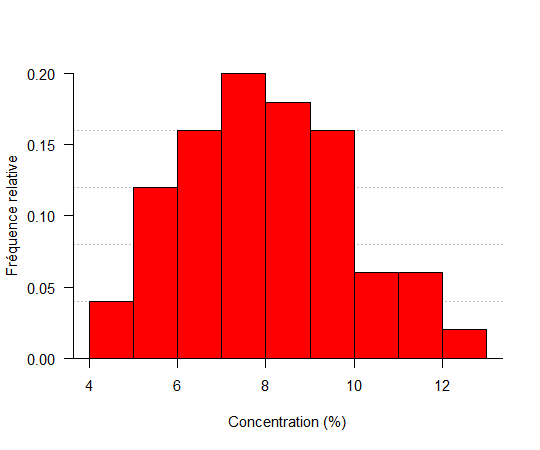
\includegraphics[width=4.8cm]{Images/Module 5/hist4.png}\hspace{1mm}ou\hspace{1mm}
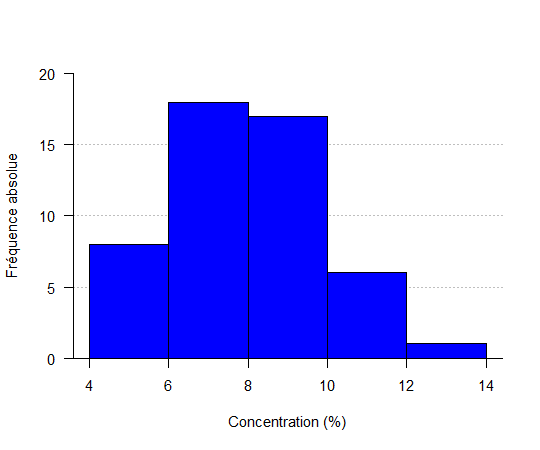
\includegraphics[width=4.8cm]{Images/Module 5/hist5.png}
\end{center}

\end{frame}


\begin{frame}[t]{Exemple 4 (suite)}

Complétons le tableau de fréquences qui définit 8 classes de valeurs.\\

\begin{tabular}{ccccc}\hline
Classe ($j$) & Largeur ($\ell_j$) & Fréq. ($n_j$) & Fréq. rel. ($f_j$) & Hauteur ($h_j$) \\ \hline
$(4,0;\, 6,0]$ & \ \     &   & \ \     \  &  \ \   \  \\[2mm]
$(6,0;\, 7,0]$ & \  \    & 8 & \  \    \  &  \ \   \  \\[2mm]
$(7,0;\, 8,0]$ &  \ \   & 10 & \  \    \  &  \ \   \  \\[2mm]
$(8,0;\, 8,5]$ & \  0,5\ & 4 & \ \ 0,08 \  &  \ \  0,16 \  \\[2mm]
$(8,5;\, 9,0]$ & \ 0,5\  & 5 & \ \ 0,10  \  & \ \  0,20 \  \\[2mm]
$(9,0;\,10,0]$ & \  1\   & 8 & \  \ 0,16 \  & \ \  0,16 \  \\[2mm]
$(10,0;\,11,0]$ & \ 1 \  & 3 & \  \ 0,06 \  & \ \  0,06 \  \\[2mm]
$(11,0;\,13,0]$ & \ 2\   & 4 & \ \ 0,08  \  & \ \  0,04 \  \\ \hline
\end{tabular}
\end{frame}
% 4,6,7,8,8.5,9,10,11,13
%$counts
%   8  8 10  4  5  8  3  4
%$density
% 0.08 0.16 0.20 0.16 0.20 0.16 0.06 0.04

\begin{frame}[t]{Histogramme avec classes de largeur inégale}

\begin{center}
  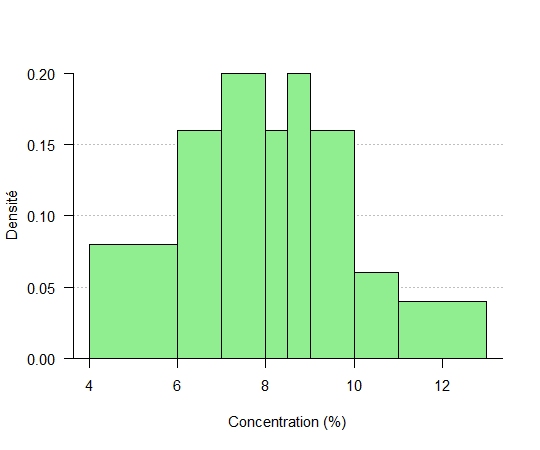
\includegraphics[width=8cm,trim= 0mm 0mm 0mm 9mm, clip]{Images/Module 5/hist6.png}  
\end{center}



\end{frame}


\subsection{Diagramme en boîte ({\em boxplot})}

\begin{frame}[t]{Diagramme en boîte}

{\small
Le \alert{diagramme en boîte}  ({\em boxplot} ou diagramme de quartiles) permet aussi d'illustrer la distribution d'une série d'observations.\\

Un diagramme en boîte a l'allure suivante:
}
\begin{center}
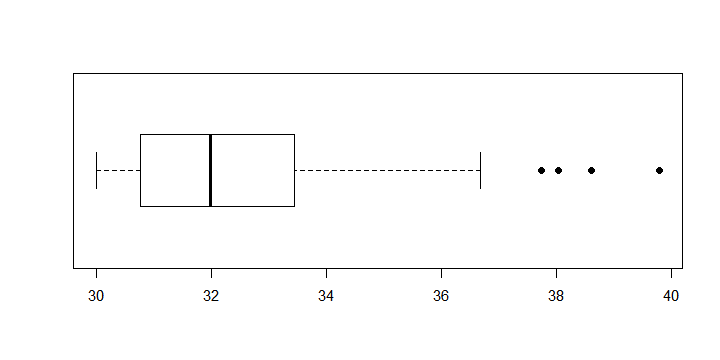
\includegraphics[width=8cm]{Images/Module 5/box-rien.png}
\end{center}
\end{frame}

\begin{frame}[t]{Procédure de construction d'un diag. en boîte}

{\small
Un diagramme en boîte peut \^etre tracé à la verticale ou à l'horizontale. Il est constitué:
\begin{itemize}
\item<1-> d'un axe gradué
\item<2-> d'une boîte aux extrémités en $Q_1=q_{0,25}$ et $Q_3=q_{0,75}$
\item<2-> d'une ligne centrale au niveau de la médiane $Q_2$
\item<3-> on calcule (\alert{on ne trace PAS}) des bornes théoriques inférieure et supérieure:
\begin{align}
b_{inf}&=q_{0,25}-1,5EIQ\label{eq:binf}\\
b_{sup}&=q_{0,75}+1,5EIQ\label{eq:bsup}
\end{align}
\item<3-> d'un trait (``moustache'') de $Q_3$ jusqu'à \alert{la plus grande valeur de l'échantillon inférieure à $b_{sup}$}

\item<3-> d'un trait (``moustache'') de $Q_1$ jusqu'à \alert{la plus petite valeur de l'échantillon supérieure à $b_{inf}$}
\end{itemize}
}
\end{frame}

\begin{frame}[t]{Procédure (suite)}

{\small
\begin{itemize}
\item<1-> de points pour chaque observation à
l'extérieur de l'intervalle $[b_{inf},b_{sup}]$
\end{itemize}
Les observations représentées par des points sur un boxplot sont parfois appelées {\em données aberrantes} ou {\em données extrêmes}, puisqu'elles sont très peu plausibles sous une loi normale.\\
\bigskip

\underline{Exercice}: Remplacez les quartiles échantillonnaux par les quartiles théoriques sous une loi $N(\mu,\sigma^2)$ dans les équations (\ref{eq:binf})-(\ref{eq:bsup}) et calculez $P(X<b_{inf}\text{\ ou\ }X>b_{sup})$ si $X\sim N(\mu,\sigma^2)$. Quelle est la probabilité d'observer une valeur extrême, i.e. hors de $[b_{inf}, \, b_{sup}]$?
}
\end{frame}
\begin{frame}[t]{Utilité du diagramme en boîte}

{\small
Le diagramme en boîte permet d'évaluer en un coup d'oeil certaines propriétés de la distribution des observations:
\begin{itemize}
\item le centre de la distribution (mesuré par la médiane);
\item la dispersion (mesurée par l'écart inter-quartile);
\item la symétrie (l'écart entre le 1er quartile et la médiane est-il le m\^eme que
l'écart entre la médiane et le 3e quartile? les moustaches sont-elles de même longueur?);
\item si certaines observations sont peu plausibles sous la loi normale (trop extrêmes);
\end{itemize}
}

 Mais surtout idéal pour comparer plusieurs échantillons simultanément (voir page suivante).
\end{frame}

\begin{frame}[t]{Diagrammes en boîte juxtaposés}

\begin{center}
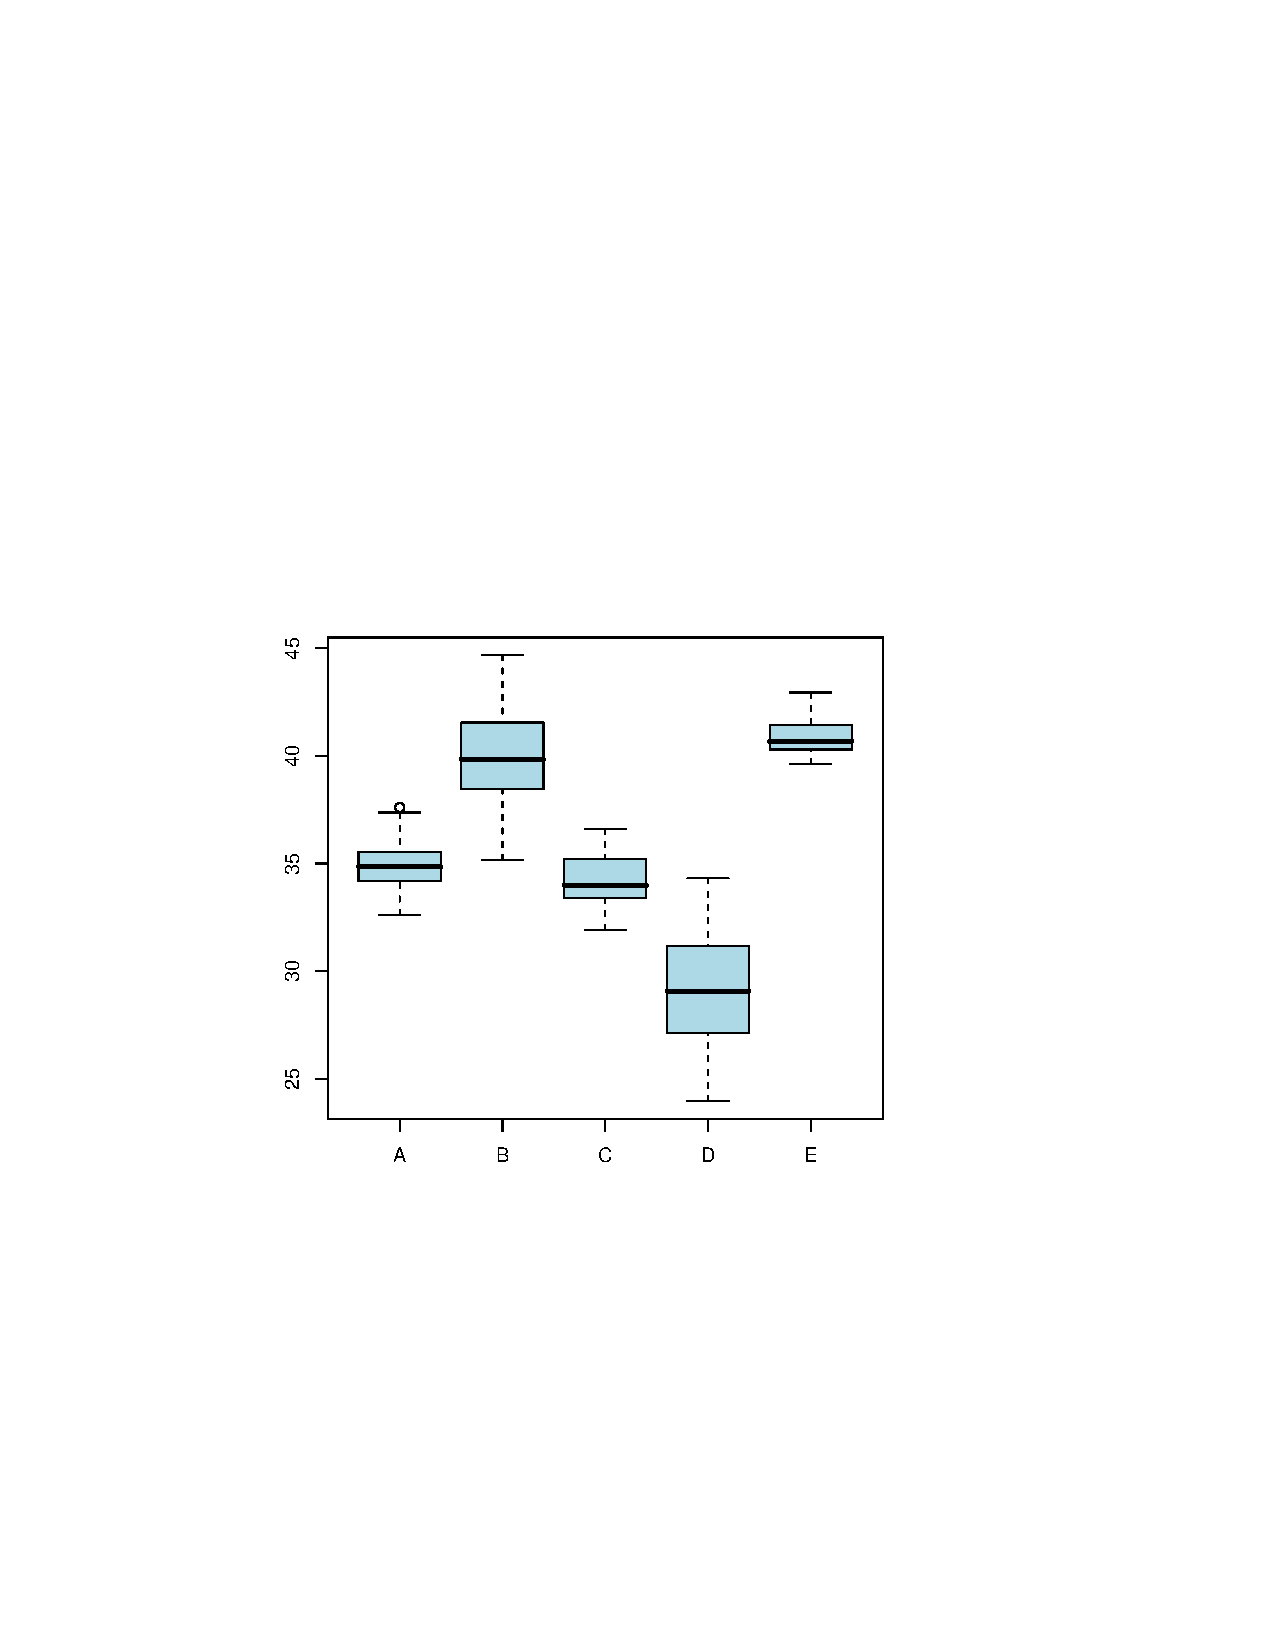
\includegraphics[width=8cm]{Images/Module 5/Diag_boite2.pdf}
\end{center}
\end{frame}

\begin{frame}[t]{Exercice (retour à l'exemple 4)}

Construire à la main le diagramme en boîte des concentrations de phosphates, et montrer qu'il a l'allure suivante:

\begin{center}
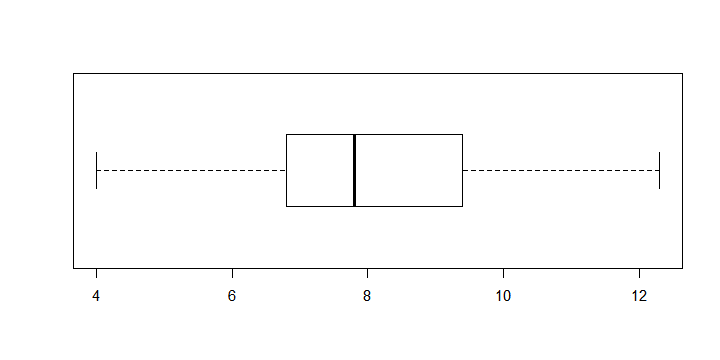
\includegraphics[width=8cm]{Images/Module 5/box-conc.png}
\end{center}
\end{frame}

\subsection{Diagramme quantile-quantile normal}
\begin{frame}[t]{Diagramme quantile-quantile normal}

\begin{itemize}\itemsep3mm
\item \underline{But}: vérifier si la loi normale est un bon modèle pour la population à l'étude
\item \underline{Principe}: les quantiles de l'échantillon sont comparés aux quantiles auxquels on s'attendrait sous une loi normale.
\item \underline{Technique} (grosso modo): on associe à chaque statistique d'ordre $x_{(i)}$ la valeur du quantile théorique normal d'ordre $i/(n+1)$.  On trace les points sur un graphique, et les points seront alignés si le modèle théorique est bon.
\end{itemize}

\end{frame}

\begin{frame}[t]{Exemple 4 des concentrations de phosphate}
\begin{center}
    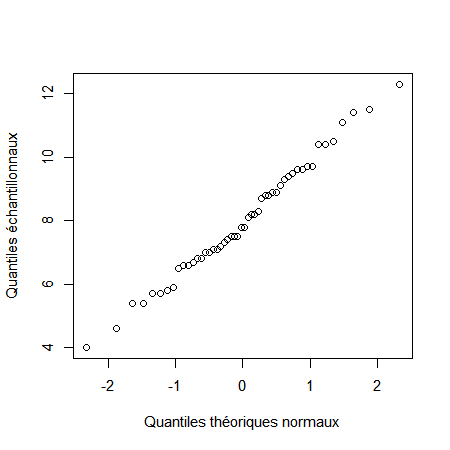
\includegraphics[width=7cm]{Images/Module 5/qq-conc.png}

\end{center}
\end{frame}

\begin{frame}[t]{Diagramme quantile-quantile normal}

\centerline{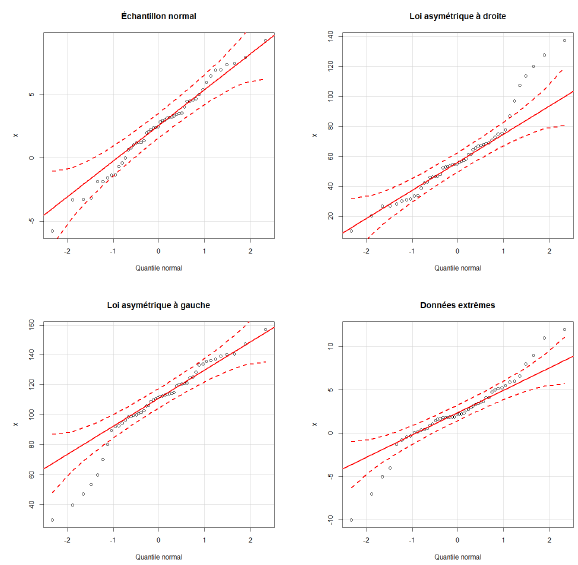
\includegraphics[width=7.5cm]{Images/Module 5/qqplot2.png}}
\end{frame}


\begin{frame}[t]{Réponses aux exemples}

{\scriptsize
\begin{enumerate}
  \item $\{x_{(1)}, x_{(2)}, x_{(3)}, x_{(4)}\}=\{2, 8, 11, 17\}$
  \item
      \begin{enumerate}[a)]
      \item $q_{0,3}=4$
      \item $q_{0,65}=7,5$
     \end{enumerate}
  \item $Q_1=2,5$, $Q_2=5$, $Q_3=14$
  \item $\mbox{ }$

  \begin{tabular}{ccccc}\hline
Classe ($j$) & Largeur ($\ell_j$) & Fréq. ($n_j$) & Fréq. rel. ($f_j$) & Hauteur ($h_j$) \\ \hline
$(4,0;\, 6,0]$ & \ 2 \   & 8 & \ \   0,16  \  &  \ \ 0,08  \  \\
$(6,0;\, 7,0]$ & \  1\   & 8 & \  \  0,16  \  &  \ \ 0,16  \  \\
$(7,0;\, 8,0]$ &  \ 1\   & 10 & \  \ 0,20   \  &  \ \ 0,20  \  \\\hline
\end{tabular}

 \end{enumerate}
 }
\end{frame}



\end{document}